\documentclass[12pt,a4paper,oneside]{article}
\usepackage{geometry}
\geometry{
	left=1.5cm, %% canh giữa hình
	right=1.5cm,
	top=2cm,
	bottom=2cm,
}
%ver-texlive2021
\usepackage{amsmath,amssymb,mathrsfs,fancyhdr,enumerate,multirow,makecell,currfile,venndiagram}
\usepackage{tikz-3dplot,tikz,tkz-tab,tabvar}
\usepackage{graphics}
\usepackage{tabularx}
\usetikzlibrary{arrows,calc,intersections,angles,snakes,quotes,backgrounds,shapes.geometric,patterns}
\usepackage{pgfplots}
\pgfplotsset{compat=1.9}
\usepgfplotslibrary{fillbetween}
\usepackage[tikz]{bclogo}
%\usepackage{xcolor}
% \usepackage{tcolorbox}
\usepackage{ex_test}
\usepackage{times}
\usepackage{array}

\setlength{\columnseprule}{1pt} 
\usepackage{tabularx,array}
\usepackage{fancyhdr}
\pagestyle{fancy}
\fancyhead{} 
\fancyfoot{} 
\fancyfoot[C]{\textbf{\thepage}/5 - Mã đề \textbf{246}} 
\renewcommand{\headrulewidth}{0pt} 
\renewcommand{\nameex}{\color{blue}Câu}

%\usepackage{xcolor}
%\usepackage{tikz}
%
%\newcommand{\circlelabel}[1]{%
%	\tikz[baseline=(c.base)] 
%	\node[draw=blue, circle, inner sep=1pt, line width=0.7pt] (c)
%	{\textcolor{blue}{#1}};%

\renewcommand{\FalseEX}{\stepcounter{dapan}\circled{\textbf{\Alph{dapan}}}}

\begin{document}
	
	% \begin{minipage}[t]{0.38\textwidth}
		% 	\begin{center}
			% 	{\large\bfseries SỞ GD\&ĐT TP. HỒ CHÍ MINH\\
				% 	TRƯỜNG THPT HỒ THỊ BI}\\%[0.6em]
			% \rule{3.6cm}{0.8pt}\\[-0.2em]
			% {\itshape (Đề kiểm tra có 02 trang)}	
			% 	\end{center}
		% \end{minipage}\hfill
	% \begin{minipage}[t]{0.45\textwidth}
		% 	\centering
		% 	{\Large\bfseries ĐỀ KIỂM TRA GIỮA HỌC KỲ 1}\\[-0.15em]
		% 	{\Large\bfseries NĂM HỌC 2025 -- 2026}\\[-0.15em]
		% 	{\Large\bfseries MÔN TOÁN -- Khối lớp 11}\\[0.25em]
		% 	{\bfseries Thời gian làm bài : 60 phút}\\[-0.15em]
		% 	{(không kể thời gian phát đề)}
		% \end{minipage}
	
\begin{center}
	\large\bfseries ĐỊNH LUẬT CHARLES (ĐẲNG ÁP)\\
	\bfseries \textcolor{red}{Trương Nguyễn Phước Tâm}
\end{center}
	
\vspace{0.2cm}
%\noindent\rule{\textwidth}{0.5pt}
\noindent\textbf{PHẦN I. Câu trắc nghiệm nhiều phương án lựa chọn.} Mỗi câu hỏi chỉ chọn một phương án.
\begin{ex}
	Quá trình biến đổi trạng thái của một khối lượng khí \dots(1)\dots khi giữ áp suất không đổi được gọi là quá trình \dots(2)\dots Điền các cụm từ thích hợp vào các chỗ trống.
	\choice
	{(1) thay đổi; (2) đẳng tích}
	{(1) xác định; (2) đẳng tích}
	{(1) thay đổi; (2) đẳng áp}
	{(1) xác định; (2) đẳng áp}
\end{ex}

\begin{ex}
	Trong hiện tượng nào sau đây có quá trình đẳng áp của một lượng khí xác định?
	\choice
	{Thổi không khí vào một quả bóng bay}
	{Quả bóng bàn bị bẹp nhúng vào nước nóng phồng lên như cũ}
	{Không khí trong một xi lanh đặt nằm ngang có áp suất bằng áp suất khí quyển bên ngoài được đun nóng thì pít-tông chuyển động thẳng đều không ma sát trong xi lanh}
	{Không khí trong một xi lanh đặt thẳng đứng được đun nóng đẩy pít-tông chuyển động nhanh dần}
\end{ex}

\begin{ex}
	\immini{Hình bên là thiết bị thí nghiệm để xác minh mối liên hệ giữa thể tích và nhiệt độ của khí khi áp suất không đổi. Sử dụng giá đỡ để cố định xilanh chứa một lượng khí nhất định và nhiệt kế trong một cốc đựng đầy nước nóng. Trong quá trình thí nghiệm, khi nhiệt độ nước giảm dần, dữ liệu về nhiệt độ và thể tích khí được ghi lại. Thao tác nào sau đây có thể giúp giảm sai số thí nghiệm?
	\choice
	{Đo và ghi lại nhiệt độ môi trường trước khi thí nghiệm}
	{Đo và ghi lại áp suất khí quyển trước khi thí nghiệm}
	{Đợi cho đến khi nhiệt độ trên nhiệt kế ổn định mới ghi dữ liệu}
	{Giữ mặt nước cao hơn đầu dưới của piston trong quá trình đo}
}{
	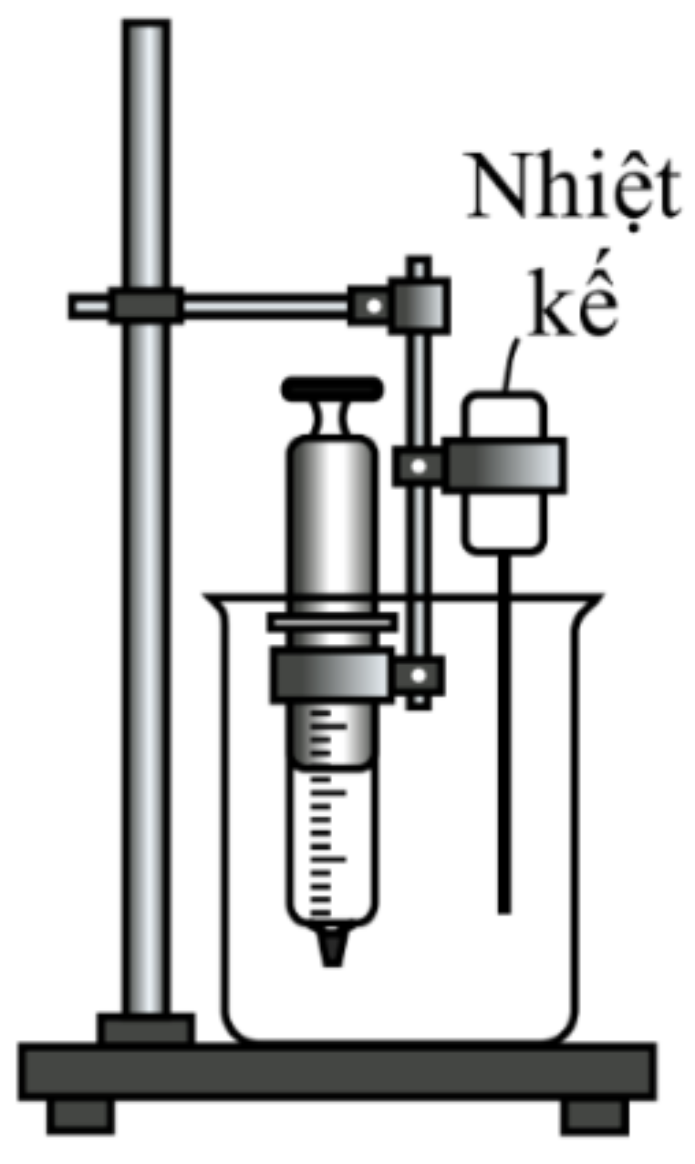
\includegraphics[scale=0.1]{img1/nhiet_ke.png}
}
\end{ex}

\begin{ex}
	Chọn câu trả lời đúng: Quá trình đẳng áp cho biết hệ thức liên hệ giữa:
	\choice
	{Thể tích và áp suất khí khi nhiệt độ không đổi}
	{Áp suất và nhiệt độ tuyệt đối khi thể tích không đổi}
	{Thể tích và nhiệt độ tuyệt đối khi áp suất không đổi}
	{Thể tích, áp suất và nhiệt độ của khí lí tưởng}
\end{ex}

\begin{ex}
	Biểu thức nào bên dưới mô tả đúng mối liên hệ giữa thể tích $V$ và nhiệt độ tuyệt đối $T$ của một chất khí lí tưởng trong quá trình đẳng áp?
	\choice
	{$V \sim \dfrac{1}{T}$}
	{$V \sim T^2$}
	{$V \sim T$}
	{$V \sim \dfrac{1}{T^2}$}
\end{ex}

\begin{ex}
	Biểu thức nào sau đây không phù hợp với nội dung của định luật đẳng áp (định luật Charles).
	\choice
	{$V/T = \text{hằng số}$}
	{$V_1/T_1 = V_2/T_2$}
	{$V = V_0(1 + \alpha t)$}
	{$V \sim 1/T$}
\end{ex}

\begin{ex}
	Gọi $\rho$ là khối lượng riêng của một chất khí lí tưởng xác định trong quá trình biến đổi đẳng áp. Biểu thức nào sau đây biểu diễn đúng mối liên hệ giữa nhiệt độ tuyệt đối $T$ và khối lượng riêng $\rho$?
	\choice
	{$\rho T = \text{hằng số}$}
	{$\rho T^2 = \text{hằng số}$}
	{$\dfrac{\rho}{T} = \text{hằng số}$}
	{$\dfrac{T}{\rho} = \text{hằng số}$}
\end{ex}

\begin{ex}
	Trong hệ toạ độ $(V, T)$, đường biểu diễn nào sau đây là đường đẳng áp?
	\choice
	{Đường thẳng song song với trục hoành}
	{Đường thẳng song song với trục tung}
	{Đường hypebol}
	{Đường thẳng kéo dài đi qua gốc toạ độ}
\end{ex}

\begin{ex}
	Đồ thị nào sau đây \textbf{không} phù hợp với quá trình đẳng áp?
	\begin{figure}[ht]
		\centering
		
\includegraphics[width=0.8\linewidth]{img1/C9.png}
		\label{fig:placeholder}
	\end{figure}
	\choice
	{Hình 1}
	{Hình 2}
	{Hình 3}
	{Hình 4}
\end{ex}

\begin{ex}
	Đường biểu diễn quá trình đẳng áp của một lượng khí xác định là \textbf{sai}?
	\begin{figure}[ht]
		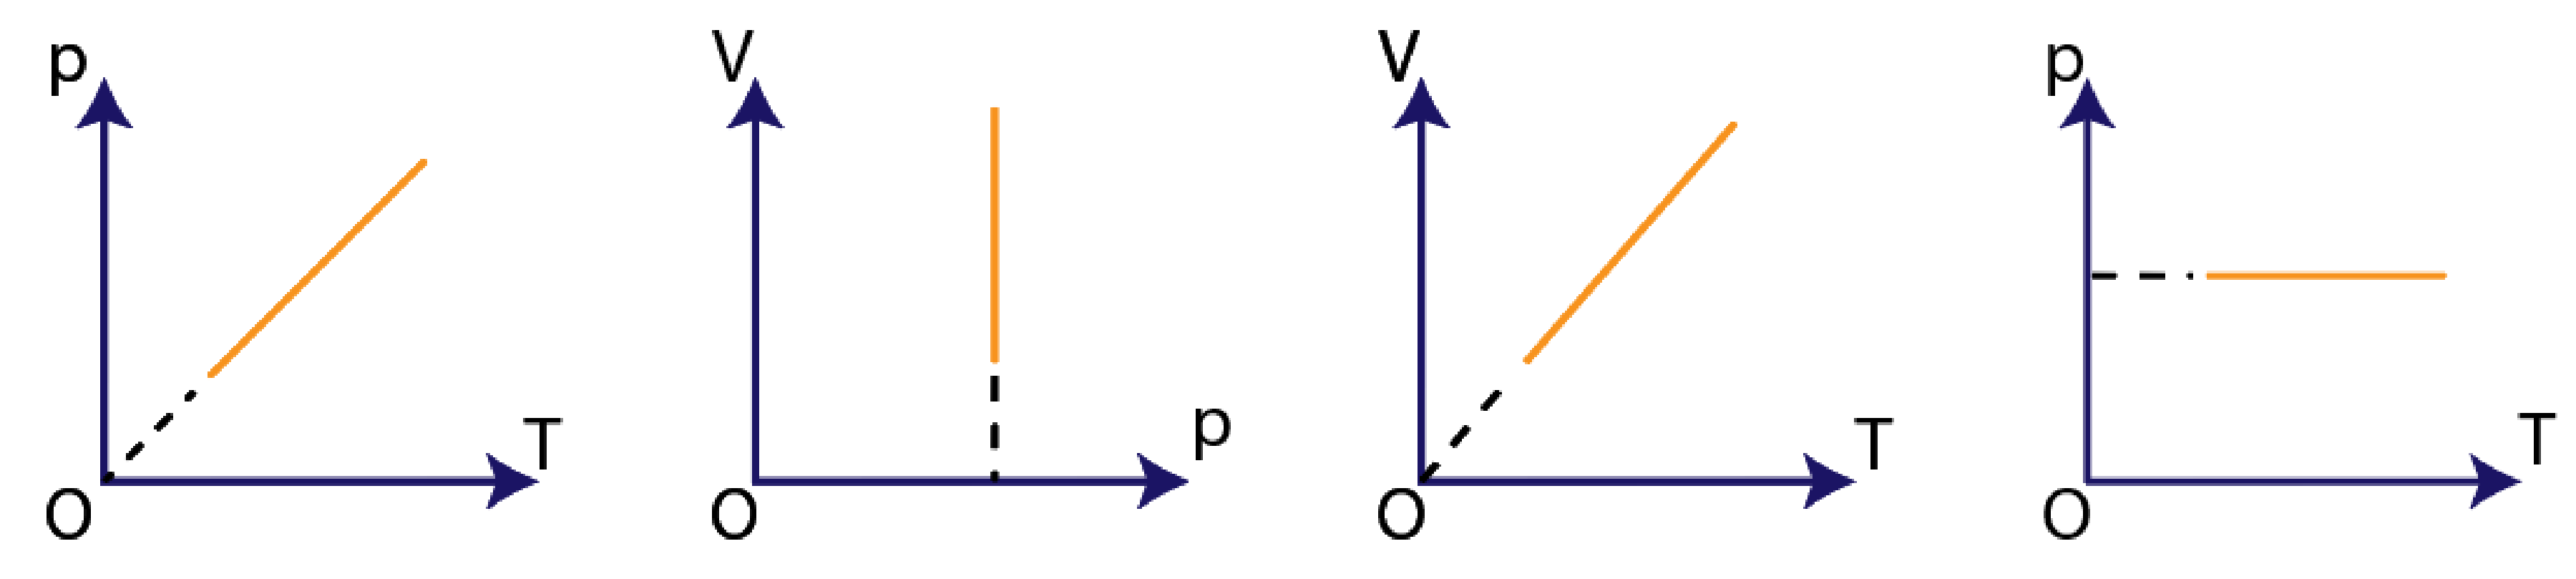
\includegraphics[width=0.9\linewidth]{img1/C10.png}
		\label{fig:placeholder}
	\end{figure}
	\vspace{-0.5cm}
	\def\dotEX{}
	\choice
	{}
	{}
	{}
	{}
\end{ex}

\begin{ex}
	Cho đồ thị biến đổi trạng thái của một khối khí lí tưởng xác định, từ trạng thái 1 đến trạng thái 2. Đồ thị nào dưới đây tương ứng với đồ thị trên biểu diễn đúng quá trình biến đổi trạng thái của khối khí này?
	\vspace{-0.75cm}
	\begin{figure}[ht]
		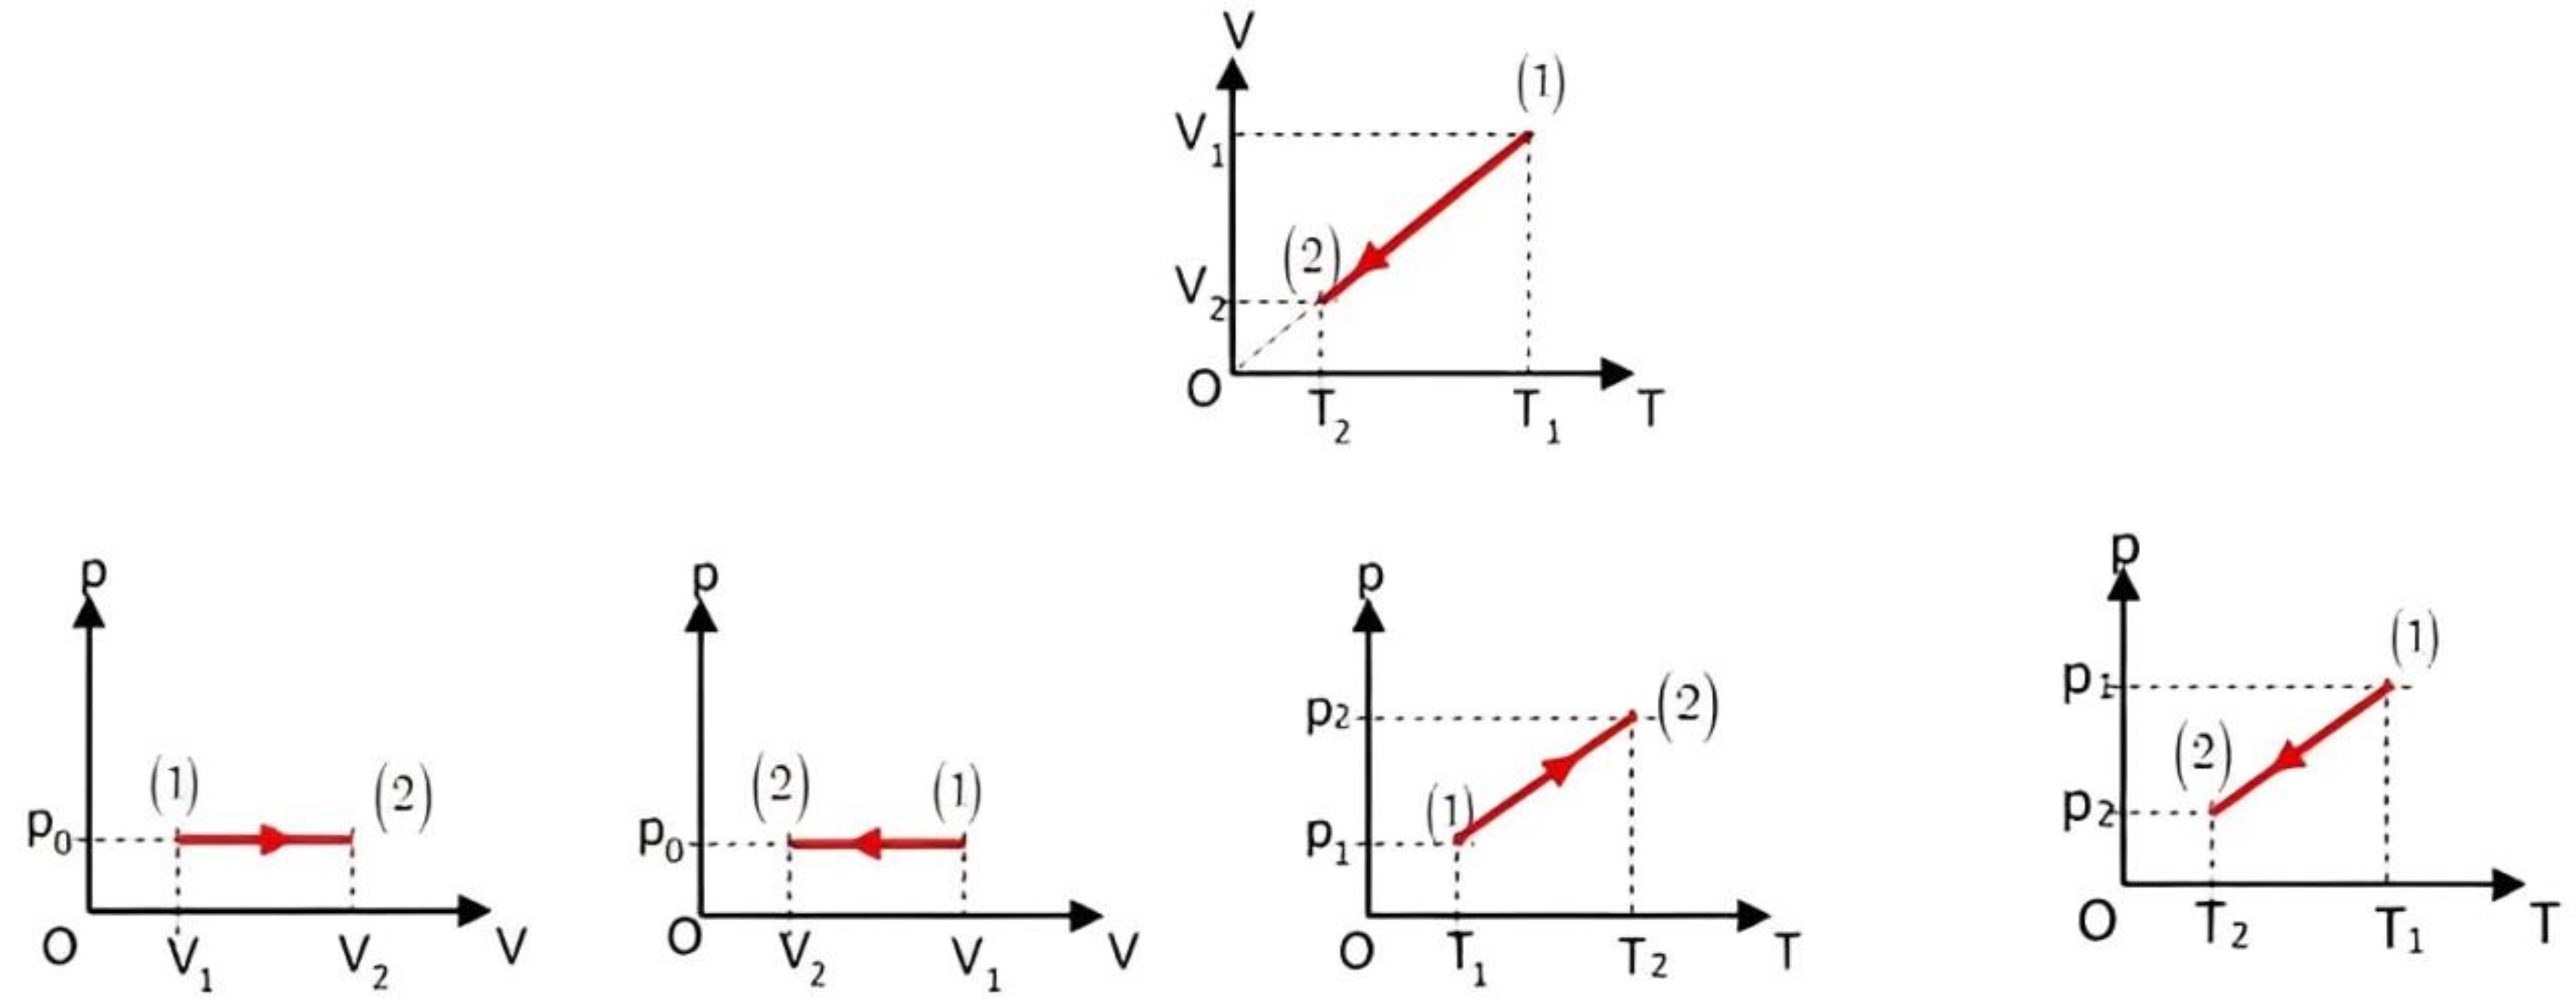
\includegraphics[width=0.95\linewidth]{img1/C11.png}
		\label{fig:placeholder}
	\end{figure}
	\vspace{-0.5cm}
	\def\dotEX{}
	\choice
	{}
	{}
	{}
	{}
\end{ex}

\begin{ex}
	\immini{
	Một giọt nước nhỏ mắc kẹt lại trong một chiếc ống nằm ngang như hình vẽ.
	}{
	\centering
	
\includegraphics[scale=0.1]{img1/C12.png}
	}
	\noindent Khi phần không khí trong ống tăng nhiệt độ (chậm) thì chất khí giãn nở từ từ đẩy giọt nước dịch chuyển sang phải. Quá trình biến đổi trạng thái của chất khí trong ống là quá trình
	\choice
	{đẳng nhiệt}
	{đẳng tích}
	{đẳng áp}
	{áp suất, nhiệt độ và thể tích đều thay đổi}
\end{ex}

\begin{ex}
	Khi thổi bong bóng xà phòng, ta quan sát thấy lúc đầu bong bóng bay lên cao rồi dần dần rơi xuống (nếu bong bóng không vỡ giữa chừng). Hãy giải thích hiện tượng và cho biết tại sao bong bóng lại rơi xuống?
	
	(1) Bong bóng xà phòng chịu tác dụng của hai lực chính: trọng lực $P$ hướng thẳng đứng xuống dưới (không đổi) và lực đẩy Acsimet của không khí $F_A$ hướng thẳng đứng lên trên.
	
	(2) Lúc đầu, khối khí trong bong bóng xà phòng có nhiệt độ cao hơn không khí (hơi thở ra của người có nhiệt độ $37^{\circ}\text{C}$) và $F_A > P$, làm cho bong bóng bay lên.
	
	(3) Sau đó, bong bóng xà phòng giảm nhiệt độ do tỏa nhiệt lượng ra không khí và thu nhỏ thể tích bong bóng lại nên $F_A$ nhỏ dần đi, còn $P$ không đổi. Đến một lúc nào đó thì $F_A < P$, kết quả là tốc độ đi lên của bong bóng giảm dần rồi từ từ rơi xuống.
	\choice[2]
	{(1) sai; (2), (3) đúng}
	{(1) đúng; (2), (3) sai}
	{(1), (2) và (3) sai}
	{(1), (2) và (3) đúng}
\end{ex}

\begin{ex}
	Ở gần nhiệt độ ngưng tụ, chúng ta không thể coi các phân tử khí \dots(1)\dots được nữa và chất khí \dots(2)\dots tuân theo định luật Boyle hay định luật Charles. Điền các cụm từ thích hợp vào các chỗ trống.
	\choice
	{(1) chuyển động hỗn loạn; (2) không còn}
	{(1) di chuyển tự do; (2) không còn}
	{(1) di chuyển tự do; (2) vẫn còn}
	{(1) chuyển động hỗn loạn; (2) vẫn còn}
\end{ex}

% ===========================================================
\noindent\textbf{PHẦN II. Câu trắc nghiệm đúng sai.} Các ý \textbf{a), b), c), d)} ở mỗi câu, chọn đúng hoặc sai.

\begin{ex}
	Một khối khí chứa $3{,}01 \cdot 10^{23}$ phân tử khí nitrogen ở nhiệt độ $27^{\circ}\text{C}$ và có khối lượng riêng $1{,}37\,\text{kg/m}^3$. Sau khi nung nóng đẳng áp khí có nhiệt độ $147^{\circ}\text{C}$.
	\choiceTF
	{Khối lượng khí nitrogen nói trên là $14\,\text{g}$}
	{Thể tích khí nitrogen) ở $27^{\circ}\text{C}$ là $10{,}22\,\text{m}^3$}
	{Thể tích của khí nitrogen) tỉ lệ thuận với nhiệt độ $t^{\circ}\text{C}$}
	{Sau khi nung nóng đẳng áp, khí có thể tích $14{,}3\,\text{dm}^3$}
\end{ex}

\begin{ex}
	Một lượng khí có thể tích $40$ lít. Nếu thể tích của một lượng khí tăng thêm $9$ lít thì nhiệt độ cũng tăng $81\,\text{K}$. Biết quá trình trên là quá trình đẳng áp. Xét tính đúng sai của các mệnh đề sau:
	\choiceTF
	{Nhiệt độ ban đầu của lượng khí là $180\,\text{K}$}
	{Nếu thể tích giảm một lượng $19$ lít thì nhiệt độ cũng giảm một lượng $171\,\text{K}$}
	{Từ trạng thái ban đầu nếu thể tích của lượng khí giảm đi $10$ lít thì nhiệt độ giảm thêm $90\,\text{K}$ so với ban đầu}
	{Khi nhiệt độ của thể khí trên là $1350\,\text{K}$ thì thể tích của nó là $15$ lít}
\end{ex}

\begin{ex}
	Một quả bóng bay được bơm khí helium đến thể tích $V_0$ ở nhiệt độ $20^{\circ}\text{C}$. Khi được mang ra ngoài trời nắng, nhiệt độ của khối khí bên trong quả bóng tăng lên đến $40^{\circ}\text{C}$. Áp suất trong quả bóng được coi như không đổi và quả bóng có khả năng dãn nở nhưng chỉ dãn nở tối đa $1{,}101$ lần thể tích ban đầu $V_0$. Coi khối khí bên trong quả bóng là khí lí tưởng.
	\choiceTF
	{Thể tích của quả bóng bay tăng tỉ lệ thuận với nhiệt độ tuyệt đối của khí helium}
	{Nếu quả bóng đi qua vùng không khí nóng có nhiệt độ $50^{\circ}\text{C}$ thì quả bóng sẽ bị vỡ}
	{Nếu cho quả bóng vào vùng nhiệt độ dưới $0^{\circ}\text{C}$ thể tích quả bóng sẽ giảm so với thể tích ban đầu}
	{Khi nhiệt độ khí helium tăng từ $20^{\circ}\text{C}$ đến $40^{\circ}\text{C}$ thể tích của quả bóng bay sẽ tăng gấp đôi}
\end{ex}

\begin{ex}
	\immini{
	Một nhóm học sinh sử dụng bình thuỷ tinh hình cầu gắn với một ống nhỏ AB có tiết diện $0{,}1\,\text{cm}^2$ trong đó có giọt thủy ngân dịch chuyển được để khảo sát quan hệ giữa các thông số trạng thái của khí trong bình. Khi khảo sát ở $20^{\circ}\text{C}$ thì giọt thuỷ ngân cách A $30\,\text{cm}$. Bỏ qua sự nở vì nhiệt của bình. Nhóm học sinh thực hiện các thao tác thí nghiệm và rút ra được các kết luận.
	}{
	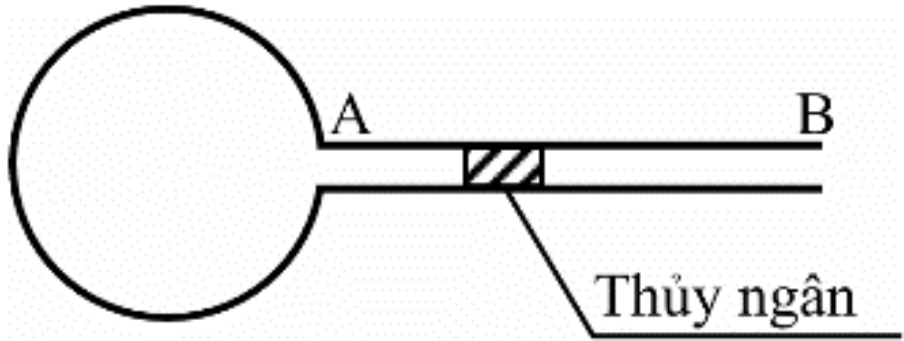
\includegraphics[scale=0.15]{img1/binh_cau.png}
	}
	\choiceTF
	{Hơ nóng khí trong bình thì giọt thuỷ ngân sẽ dịch chuyển lại gần đầu A}
	{Vì không có sự nở vì nhiệt của bình nên quá trình biến đổi trạng thái của khối khí khi bị hơ nóng là quá trình đẳng tích}
	{Hơ nóng khí trong bình thì giọt thủy ngân sẽ dịch chuyển về phía B đến khi áp suất của khí trong bình cân bằng với áp suất khí quyển}
	{Khi nhiệt độ của khí được hơ nóng đến $25^{\circ}\text{C}$ thì giọt thuỷ ngân cách A $50\,\text{cm}$. Phần thể tích của khí chứa trong bình thủy tinh hình cầu là $114{,}2\,\text{cm}^3$}
\end{ex}

\begin{ex}
	Một bình có dung tích $140\,\text{cm}^3$ chứa không khí ở nhiệt độ $147^{\circ}\text{C}$ nối với một ống nằm ngang chứa đầy thuỷ ngân, đầu kia thông với khí quyển. Không khí trong bình được làm lạnh đến $27^{\circ}\text{C}$, coi dung tích bình không đổi và khối lượng riêng của thuỷ ngân là $13{,}6\,\text{g/cm}^3$.
	\choiceTF
	{Ban đầu, cột thuỷ ngân trong ống nằm ngang cân bằng. Áp suất trong bình bằng với áp suất khí quyển}
	{Khi vừa mới giảm nhiệt độ của không khí trong bình, áp suất trong bình giảm và nhỏ hơn áp suất khí quyển làm cho thuỷ ngân bị đẩy vào chiếm một phần thể tích bình chứa}
	{Thể tích của khí sau khi thuỷ ngân chảy vào bình là $100\,\text{cm}^3$}
	{Khối lượng thuỷ ngân chảy vào bình $544$ gam}
\end{ex}

\begin{ex}
	Một ống thuỷ tinh hình trụ thẳng đứng có tiết diện ngang nhỏ, đầu trên hở, đầu dưới kín. Ống chứa một khối khí (coi là khí lí tưởng) có chiều cao $L = 90\,\text{cm}$ được ngăn cách với bên ngoài bởi một cột thuỷ ngân có độ cao $h = 75\,\text{cm}$, mép trên cột thuỷ ngân cách miệng trên của ống một đoạn $l = 10\,\text{cm}$. Nhiệt độ ban đầu của khí trong ống là $t_0 = -3^{\circ}\text{C}$, áp suất khí quyển là $p_0 = 75\,\text{cmHg}$. Người ta thay đổi chậm nhiệt độ của khí trong ống để cột thủy ngân có thể di chuyển trong ống thủy tinh.
	\choiceTF
	{Khi cột thủy ngân chưa trào ra ngoài thì quá trình biến đổi của khí trong ống là quá trình đẳng áp}
	{Đưa nhiệt độ của khí trong ống đến $27^{\circ}\text{C}$ thì mép trên của cột thuỷ ngân vừa chạm miệng trên của ống}
	{Khi được làm nóng, cột thủy ngân sẽ dịch chuyển về phía đầu dưới của ống}
	{Để thuỷ ngân trong ống tràn hết ra ngoài thì phải đưa nhiệt độ của khí trong ống đến nhiệt độ $262{,}5\,\text{K}$}
\end{ex}

\begin{ex}
	Để khảo sát mối liên hệ giữa thể tích và nhiệt độ của một lượng khí xác định khi giữ áp suất không đổi người ta bố trí thí nghiệm như hình vẽ. Cho biết áp kế có đơn vị đo Bar ($1\,\text{Bar} = 10^5\,\text{Pa}$). Cảm biến nhiệt được đặt trong nước. Đổ nước nóng vào hộp chứa để xilanh ngập hoàn toàn trong nước. Dịch chuyển pittong thật chậm, sao cho số chỉ của áp kế không đổi. Kết quả đo giá trị của phần thể tích chứa khí và nhiệt độ sau mỗi phút được ghi lại ở bảng số liệu.\\
	\begin{minipage}[t]{0.55\textwidth}
		\resizebox{\linewidth}{!}{%
		\begin{tabular}{|c|>{\centering\arraybackslash}m{4cm}|>{\centering\arraybackslash}m{4cm}|}
			\hline
			Lần đo & Nhiệt độ của khí trong xilanh $t(^{\circ}\text{C})$ & Thể tích khí trong xilanh $V(\text{ml})$ \\
			\hline
			1 & 45 & 75 \\
			\hline
			2 & 41 & 74 \\
			\hline
			3 & 37 & 73 \\
			\hline
			4 & 32 & 72 \\
			\hline
			5 & 28 & 71 \\
			\hline
		\end{tabular}
		}
	\end{minipage}
	\begin{minipage}{0.4\textwidth}
		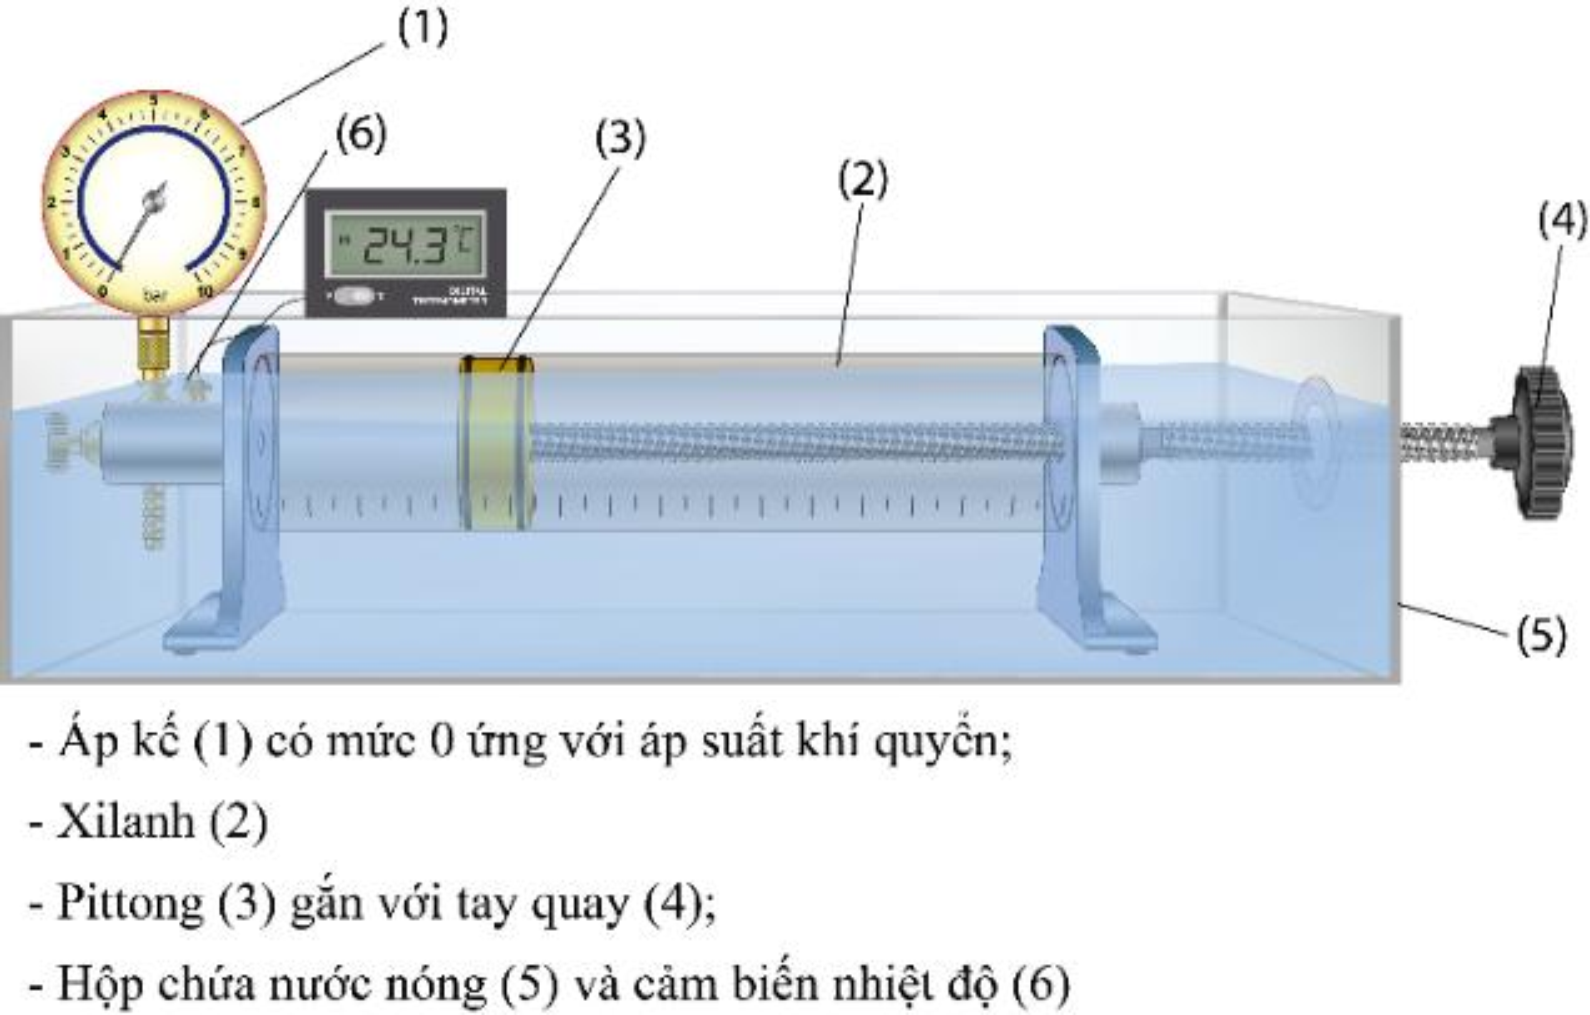
\includegraphics[scale=0.15]{img1/thi_nghiem.png}
	\end{minipage}
	\choiceTF
	{Từ bảng số liệu, ta kết luận thể tích của khối khí chứa trong xilanh tỉ lệ thuận với nhiệt độ $^{\circ}\text{C}$}
	{Trong quá trình thực hiện thí nghiệm cần chú ý khi đổ nước nóng vào hộp chứa để xilanh ngập hoàn toàn trong nước nóng và đợi một thời gian để đảm bảo nhiệt độ khối khí trong xilanh cân bằng với nhiệt độ của nước}
	{Đồ thị biểu diễn sự phụ thuộc của thể tích $V$ vào nhiệt độ $t(^{\circ}\text{C})$ trong hệ trục toạ độ $(OtV)$ là đường thẳng cắt trục $Ot$ tại điểm có nhiệt độ xấp xỉ $-273^{\circ}\text{C}$}
	{Với kết quả thu được ở bảng trên, công thức liên hệ giữa thể tích theo nhiệt độ tuyệt đối là $V \approx 0{,}24T$ phù hợp với định luật Charles}
\end{ex}

\begin{ex}
	Có thể sử dụng bộ thí nghiệm (hình bên) để tìm hiểu về mối liên hệ giữa nhiệt độ và thể tích của một lượng khí xác định khi giữ áp suất của khí không đổi.	Kết quả thí nghiệm được ghi lại như bảng bên dưới:
	\begin{center}
		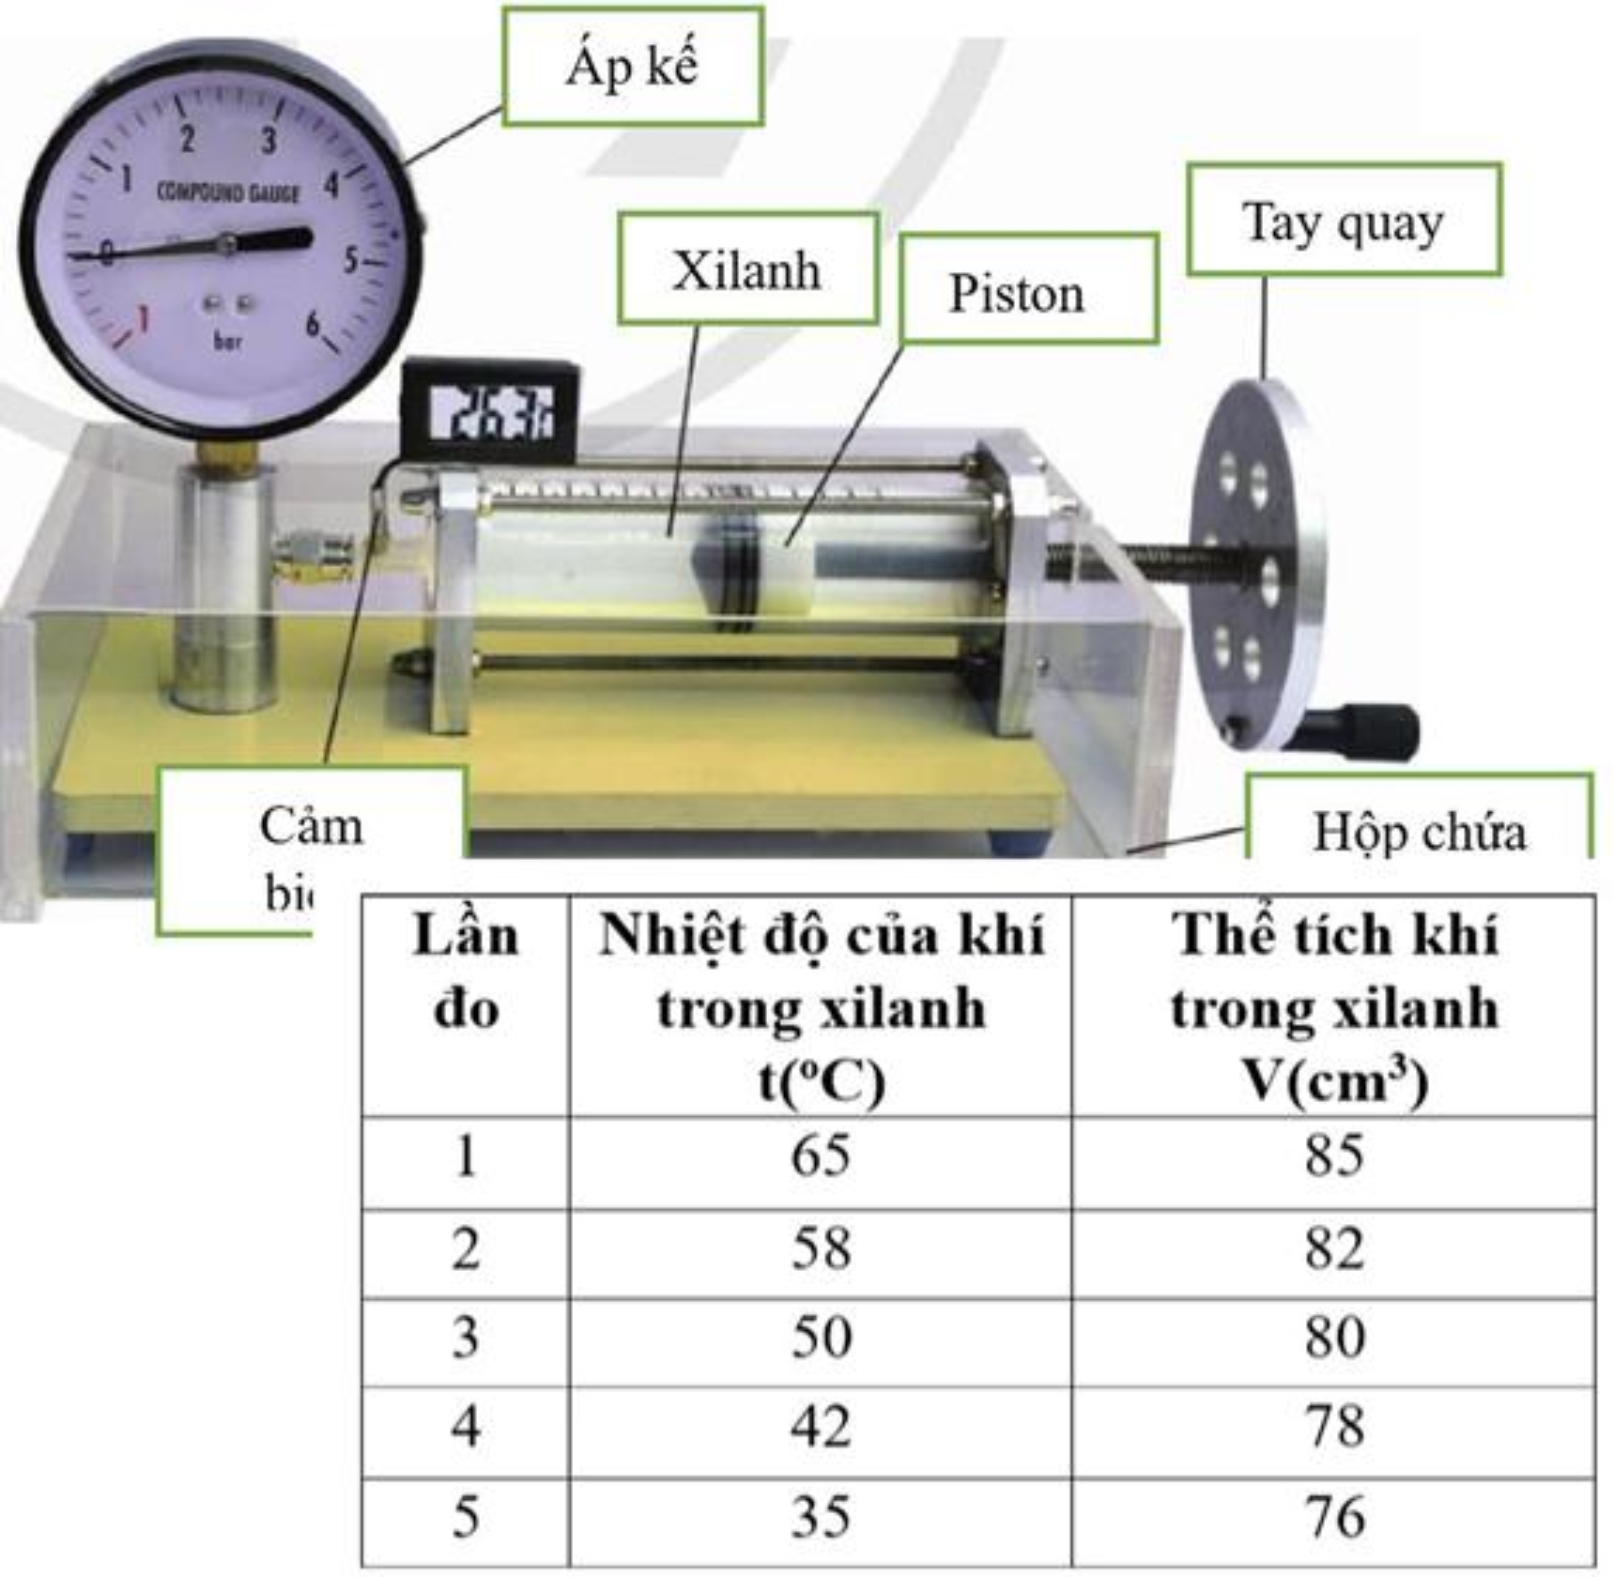
\includegraphics[scale=0.12]{img1/thi_nghiem_2.png}
	\end{center}
%	\begin{center}
%		\begin{tabular}{|c|c|c|}
%			\hline
%			Lần đo & Nhiệt độ của khí trong xilanh $t(^{\circ}\text{C})$ & Thể tích khí trong xilanh $V(\text{cm}^3)$ \\
%			\hline
%			1 & 65 & 85 \\
%			\hline
%			2 & 58 & 82 \\
%			\hline
%			3 & 50 & 80 \\
%			\hline
%			4 & 42 & 78 \\
%			\hline
%			5 & 35 & 76 \\
%			\hline
%		\end{tabular}
%	\end{center}
	\choiceTF
	{Trình tự thí nghiệm:\\
		+ Mở van áp kế, dùng tay quay dịch chuyển piston để lấy một lượng khí xác định.\\
		+ Đổ nước nóng vào hộp chứa nước sao cho xilanh ngập hoàn toàn trong nước.\\
		+ Khi nhiệt độ không tăng nữa, đóng van áp kế, ghi giá trị thể tích và áp suất của khí.\\
		+ Sau khoảng 5 phút, dịch chuyển piston để áp suất trở lại giá trị ban đầu, ghi giá trị thể tích và nhiệt độ của khí.\\
		+ Làm lại bước cuối cùng một số lần nữa và ghi kết quả như bảng bên}
	{Thí nghiệm này kiểm chứng được định luật Charles}
	{Với kết quả thu được ở bảng trên, tỉ số giữa thể tích và nhiệt độ là $\dfrac{V}{T} = 1{,}6$ ($V$ đo bằng $\text{cm}^3$, $T$ đo bằng $\text{K}$)}
	{Thể tích lượng khí trong xilanh khi ở nhiệt độ phòng $25^{\circ}\text{C}$ là $32\,\text{cm}^3$}
\end{ex}

\end{document}